\documentclass[a4paper,
fontsize=11pt,
%headings=small,
oneside,
numbers=noperiodatend,
parskip=half-,
bibliography=totoc,
final
]{scrartcl}

\usepackage[babel]{csquotes}
\usepackage{synttree}
\usepackage{graphicx}
\setkeys{Gin}{width=.4\textwidth} %default pics size

\graphicspath{{./plots/}}
\usepackage[ngerman]{babel}
\usepackage[T1]{fontenc}
%\usepackage{amsmath}
\usepackage[utf8x]{inputenc}
\usepackage [hyphens]{url}
\usepackage{booktabs} 
\usepackage[left=2.4cm,right=2.4cm,top=2.3cm,bottom=2cm,includeheadfoot]{geometry}
\usepackage{eurosym}
\usepackage{multirow}
\usepackage[ngerman]{varioref}
\setcapindent{1em}
\renewcommand{\labelitemi}{--}
\usepackage{paralist}
\usepackage{pdfpages}
\usepackage{lscape}
\usepackage{float}
\usepackage{acronym}
\usepackage{eurosym}
\usepackage{longtable,lscape}
\usepackage{mathpazo}
\usepackage[normalem]{ulem} %emphasize weiterhin kursiv
\usepackage[flushmargin,ragged]{footmisc} % left align footnote
\usepackage{ccicons} 
\setcapindent{0pt} % no indentation in captions

%%%% fancy LIBREAS URL color 
\usepackage{xcolor}
\definecolor{libreas}{RGB}{112,0,0}

\usepackage{listings}

\urlstyle{same}  % don't use monospace font for urls

\usepackage[fleqn]{amsmath}

%adjust fontsize for part

\usepackage{sectsty}
\partfont{\large}

%Das BibTeX-Zeichen mit \BibTeX setzen:
\def\symbol#1{\char #1\relax}
\def\bsl{{\tt\symbol{'134}}}
\def\BibTeX{{\rm B\kern-.05em{\sc i\kern-.025em b}\kern-.08em
    T\kern-.1667em\lower.7ex\hbox{E}\kern-.125emX}}

\usepackage{fancyhdr}
\fancyhf{}
\pagestyle{fancyplain}
\fancyhead[R]{\thepage}

% make sure bookmarks are created eventough sections are not numbered!
% uncommend if sections are numbered (bookmarks created by default)
\makeatletter
%\renewcommand\@seccntformat[1]{}
\makeatother

% typo setup
\clubpenalty = 10000
\widowpenalty = 10000
\displaywidowpenalty = 10000

\usepackage{hyperxmp}
\usepackage[colorlinks, linkcolor=black,citecolor=black, urlcolor=libreas,
breaklinks= true,bookmarks=true,bookmarksopen=true]{hyperref}
\usepackage{breakurl}

%meta
%meta

\fancyhead[L]{K. Schuldt\\ %author
LIBREAS. Library Ideas, 39 (2021). % journal, issue, volume.
\href{https://doi.org/10.18452/23446}{\color{black}https://doi.org/10.18452/23446}
{}} % doi 
\fancyhead[R]{\thepage} %page number
\fancyfoot[L] {\ccLogo \ccAttribution\ \href{https://creativecommons.org/licenses/by/4.0/}{\color{black}Creative Commons BY 4.0}}  %licence
\fancyfoot[R] {ISSN: 1860-7950}

\title{\LARGE{Automatisierung in Wissenschaftlichen Bibliotheken der 1960er Jahre: Der Anfang des Einsatzes von Computern in Bibliotheken im DACH-Raum}}% title
\author{Karsten Schuldt} % author

\setcounter{page}{1}

\hypersetup{%
      pdftitle={Automatisierung in Wissenschaftlichen Bibliotheken der 1960er Jahre: Der Anfang des Einsatzes von Computern in Bibliotheken im DACH-Raum},
      pdfauthor={Karsten Schuldt},
      pdfcopyright={CC BY 4.0 International},
      pdfsubject={LIBREAS. Library Ideas, 39 (2021).},
      pdfkeywords={Wissenschaftliche Bibliotheken, Computer, Automatisierung, Deutschland, Österreich, Schweiz},
      pdflicenseurl={https://creativecommons.org/licenses/by/4.0/},
      pdfcontacturl={http://libreas.eu},
      baseurl={https://doi.org/10.18452/23446},
      pdflang={de},
      pdfmetalang={de}
     }



\date{}
\begin{document}

\maketitle
\thispagestyle{fancyplain} 

%abstracts
\begin{abstract}
\noindent
\textbf{Kurzfassung:} Computer wurden in den Wissenschaftlichen Bibliotheken des DACH-Raumes
in den 1960er Jahren eingeführt. Der Text vollzieht dies nach und zeigt
unter anderem, dass die Grundprobleme, die am Ende mit den
Rechenmaschinen gelöst werden sollten, zuvor auch anders angegangen
wurden. Es ging um die Beherrschung einer wachsenden Anzahl von
Literatur. Auffällig an der Geschichte ist, dass die Entwicklungen sich
relativ schnell vollzogen, dass sie im DACH-Raum relativ ähnlich
verliefen und das es nicht per se um die Einführung von Technik, sondern
um das Lösen von Problemen ging.
\end{abstract}

\begin{center}\rule{0.5\linewidth}{0.5pt}\end{center}

%body

\begin{quote}
\enquote{Hier noch einmal auf die Sorgen und Nöte der Bibliothek eingehen zu
wollen, hieße wohl Eulen nach Athen tragen. Ist doch in letzter Zeit oft
genug die Notwendigkeit diskutiert worden, durch geeignete Maßnahmen der
manchmal geradezu verzweifelten arbeitsmäßigen Situation in den
Bibliotheken abzuhelfen. Dabei stehen nicht nur allgemeine Maßnahmen der
Rationalisierung, sondern auch speziell die Automatisierung
verschiedener Arbeitsvorgänge mit entsprechenden Geräten im Mittelpunkt
des Interesses.} (Schulte-Tigges 1963: 331)
\end{quote}

\hypertarget{einleitung}{%
\section{Einleitung}\label{einleitung}}

\enquote{Mechanisierte Datenverarbeitungsverfahren}, so schrieb Walter
Lingenberg 1969, \enquote{werden in deutschen Bibliotheken erst seit wenigen
Jahren angewendet.} (Lingenberg 1969: 1) Gleichwohl stellte er in dem
Text, aus welchem diese Aussage stammt, die Ergebnisse einer Umfrage zum
Einsatz von Computern vor, bei der immerhin 22 Bibliotheken aus der BRD
-- die meisten davon, aber nicht alle, Universitätsbibliotheken --
antworteten. Diese hatten den Einsatz dieser Geräte nicht nur angedacht,
sondern waren ihn schon angegangen. Planungen gab es weit mehr, auch
schon erste Enttäuschungen über die tatsächlichen Möglichkeiten dieser
frühen Computer. (Lingenberg 1969: 9; Lingenberg 1968: 179; Pflug 1969)

Der Beitrag von Lingenberg war kein Ausreisser. Vielmehr war das Thema
Ende der 1960er Jahre im gesamten DACH-Raum präsent: Viele Bibliotheken
setzten Computer ein -- damals bekanntlich vor allem Mainframe-Rechner
in Raumgrösse, obwohl in diesem Jahrzehnt auch erste eigenständige
Geräte für den Einsatz in Büros entwickelt wurden. Viele mehr planten
dies und in den 1970ern waren Computer in Bibliotheken dann so sehr
etabliert, dass die Zahl der Beiträge zum Thema und die Anzahl der
Einrichtungen, die sich damit befassten, explodierte. Für die DDR
stellte zum Beispiel im gleichen Jahr, in dem Lingenbergs Text erschien,
Renate Ludwig (1969) die Gründung einer Arbeitsgruppe \enquote{EDAV
{[}Elektronische Datenverarbeitung, K.S.{]} in Bibliotheken} vor, die
aufgrund eines Ministerratsbeschlusses von 1967 beim Ministerium für
Hoch- und Fachschulwesen eingerichtet wurde und als Aufgabe die Planung
des Einsatzes von Computern für das gesamte Hochschul-Bibliothekswesen
des Landes übertragen bekam. In Österreich war schon 1966 ein der
Nationalbibliothek nahestehender Verein, das \enquote{Institut für
Bibliotheksforschung} gegründet worden, welcher unter anderem den
Einsatz von Computern forschend und beratend fördern sollte. (Mayerhöfer
1966; Stummvoll \& Mayerhöfer 1972; Mayerhöfer 1982) 1970 wurde in der
\enquote{Generalversammlung der Schweizer Bibliothekare} ausführlich über ein
Seminar der UNESCO in Regensburg zu diesem Thema berichtet. Dieser, auch
publizierte, Vortrag führte tief in das bis dahin vorhandene, dann schon
recht breite Wissen zum Thema ein. (Wegmüller \& Hoffmann-La Roche 1970)
Im gleichen Jahr wurden in der (damals einzigen) schweizerischen
bibliothekarischen Fachzeitschrift auch über den Stand des Einsatzes von
Computern in der Sowjetunion (Jordi 1970) und den USA (Sydler 1970)
berichtet.

Obwohl in vielen dieser Beiträge betont wurde, dass der Einsatz von
Computern nur langsam vorankommen würde und auch Überzeugungsarbeit
unter den Kolleg*innen zu leisten wäre (Schwarz 1967; Lingenberg 1969;
Pflug 1969), finden sich zumindest publiziert kaum Beiträge, welche
diese Entwicklung kritisieren würden.\footnote{Ausnahme ist ein Beitrag
  von Paul Scherrer-Bylund, immerhin bis 1962 Direktor der Bibliothek
  der ETH Zürich, aber bei Erscheinen des Artikels schon im Ruhestand.
  (Scherrer-Bylund 1969) Er greift auf eine recht anti-modernistische
  Haltung zurück, wenn er \enquote{Tradition und Technik in Bibliotheken}
  gegenüberstellt. Gleichzeitig liest sich der gesamte Text in
  Terminologie und Weitschweifigkeit wie aus der Zeit gefallen. Dies
  vermittelt den Eindruck, als wäre der Einsatz von Computern auch Teil
  eines Generationenwechsels im Bibliothekswesen im DACH-Raum gewesen.
  (Den Rückgang der \enquote{Modernekritik} und einen Generationenwechsel Ende
  der 1960er beschreibt auch Kuttner (2018).)} Wenn, dann finden sich
eher Ermahnungen dazu, die tatsächlichen Möglichkeiten und die
Geschwindigkeit der Veränderungen nicht zu überschätzen. (Baer 1964;
Stummvoll 1969) Dabei war die Entwicklung erstaunlich schnell (wie auch
andere Veränderungen in den 1960er Jahren in den Gesellschaften im
DACH-Raum). Dass der Einsatz von Computern in Bibliotheken 1969 schon
als Tatsache angesehen werden konnte, bei dem es praktisch nur noch um
die Frage ging, wann alle Einrichtungen Zugang zu einem haben würden
(Pflug 1969), ist das Ergebnis einer rasanten Entwicklung im
Bibliothekswesen. Die ganzen 1960er Jahre über wurden in den vier
genannten Ländern\footnote{Zum Fürstentum Liechtenstein, auch Teil des
  DACH-Raumes, liegen keine Publikationen zu diesem Thema vor. Das ist
  allerdings nicht überraschend, die Landesbibliothek wurde erst 1961
  gegründet, ebenso die Vorläufereinrichtung der heutigen Universität
  Liechtenstein (die erst 1992 zur Fachhochschule und 2011 zur
  Universität erhoben wurde). Insoweit fehlten im Fürstentum wohl auch
  grosse Bibliotheken, welche diese Diskussionen hätten vorantreiben
  können. Zu den Forschungsbibliotheken in den Betrieben der
  spezialisierten Industrien -- die in den anderen Ländern, gerade der
  Schweiz (Margot \& Monnier 1968), ebenfalls zum Teil früh über den
  Einsatz von Computern nachdachten -- im Fürstentum fehlen leider
  Publikationen.} über Rationalisierung und Automatisierung der Arbeit
in Bibliotheken nachgedacht -- mit, wie sich zeigen wird, auch
unterschiedlichen Ansätzen --, wobei zu Beginn des Jahrzehnts nicht klar
war, welche Rolle Maschinen in dieser Rationalisierung spielen würden.

Im vorliegenden Beitrag werden der Kontext und der Beginn des Einsatzes
von Maschinen zur Datenverarbeitung (als solche wurden Computer am Ende
der 1960er Jahre vor allem begriffen) auf der Basis von publizierten
Beiträgen dargestellt. Im folgenden Kapitel (2) wird der Kontext dieser
Entwicklungen geschildert: Warum machten sich Bibliotheken darum
Gedanken, wie sie ihre Arbeit rationeller organisieren konnten? Warum
richteten sie ihren Blick dabei auf Maschinen? Daran anschliessend
werden die Themen diskutiert, auf die sich dabei die Beiträge und
praktischen Versuche von Bibliotheken richteten (3). Hier wird sich
zeigen, dass nicht die gesamte Bibliothek oder die Nutzer*innen im Fokus
standen, sondern immer wieder über einzelne, abgrenzbare
Funktionsbereiche der bibliothekarischen Arbeit nachgedacht wurde.
Abschliessend wird auf das Fehlen von Kritiken und Utopien (4) im
Zusammenhang mit der Einführung von Computer eingegangen, welches --
angesichts anderer Veränderungen und Utopien, die sich zumindest in der
bundesdeutschen, schweizerischen und österreichischen Gesellschaft zu
dieser Zeit virulent waren -- erstaunt. Auch wenn der DACH-Raum in
diesem Beitrag gemeinsam behandelt wird, wird in einem kurzen Kapitel
auf die Unterschiede zwischen zwei Ländern, der DDR und der BRD,
eingegangen (5). Hier zeigt sich am Beispiel der Einführung von
Computern, dass, trotz gegenseitiger Einflüsse, die Entwicklung der
Bibliothekswesen jeweils länderspezifische Eigenheiten hatte. Zuletzt
wird im Fazit diskutiert, welche Bedeutung diese Geschichte für heutige
Bibliotheken hat. (6)

\begin{figure}
\centering
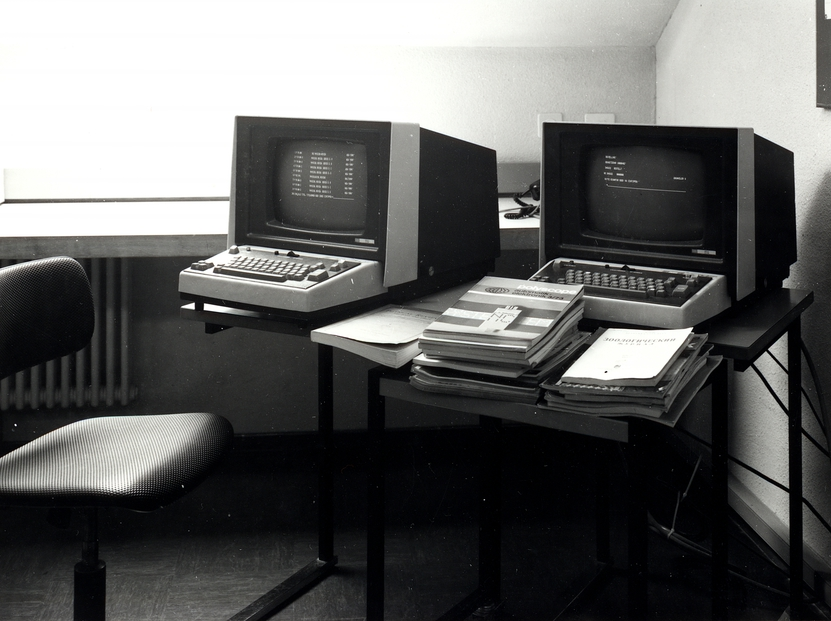
\includegraphics[width=.7\textwidth]{img/ETHZuerich01.jpg}
\caption{G. Nigg: \enquote{Zürich, ETH Zürich, Hauptgebäude
(HG), Hauptbibliothek, Zeitschriftenabteilung}, laut Metadaten 1968,
eher frühe 1970er Jahre (e-pics, ETH Zürich, \href{https://creativecommons.org/licenses/by-sa/4.0/}{CC BY-SA 4.0},
\url{http://doi.org/10.3932/ethz-a-000014445}). Terminale, die an einen
Grossrechner angeschlossen waren, genutzt für die Katalogisierung.}
\end{figure}

\hypertarget{warum-bibliotheksarbeit-rationalisieren}{%
\section{Warum Bibliotheksarbeit
rationalisieren?}\label{warum-bibliotheksarbeit-rationalisieren}}

Schon in den beginnenden 1960er Jahren herrschte im Bibliothekswesen --
und nicht nur dort -- die Überzeugung vor, dass sich die materielle
Basis der Gesellschaften radikal ändern würde. Während Grundbedürfnisse
gesichert und durch die Wirtschaftsentwicklung in Zukunft gedeckt wären,
würde die Bedeutung der Wissenschaft und die Übertragung
wissenschaftlicher Erkenntnisse in die Gesellschaft -- oft dargestellt
als die Zeit zwischen der Erfindung eines Gerätes und dessen
massenhafter Verbreitung -- eine immer weiter wachsende Bedeutung
erhalten. (Höhne 1963; Schulte-Tigges 1965) Die Wissenschaft würde immer
mehr Wissen und damit auch immer mehr Publikationen produzieren, die
Wirtschaft und Gesellschaft würde immer mehr Interesse daran entwickeln,
möglichst schnell, genau und zielgerichtet über den Fortschritt dieses
Wissens informiert zu werden. (Pietsch 1962; Rittberger 1964) Über die
Jahre treten auch weitere, mit diesen Veränderungen einhergehende,
Begründungen hinzu, beispielsweise die steigenden Studierendenzahlen und
die Hochschulreformen in der BRD. (Fock 1967)

Für die DDR stellt Höhne 1963 folgendes fest, um daraus anschliessend
abzuleiten, dass sich mit der Rationalisierung der bibliothekarischen
Arbeit befasst werden muss:

\begin{quote}
\enquote{Die ständig wachsenden Aufgaben, die heute der Lehre und Forschung
sowie der Praxis zur Erfüllung der umfangreichen wissenschaftlichen,
ökonomischen und politischen Ziele (z.B. die Erreichung des
wissenschaftlich-technischen Höchststandes) gestellt werden, fordern
auch von den Mitarbeitern der wissenschaftlichen Bibliotheken eine
kontinuierliche und termingerechte Betreuung und Versorgung aller
Bedarfsträger mit der neuesten Literatur. Nun findet aber die stürmische
Entwicklung der Wissenschaften einen Ausdruck in einem enormen Anstieg
literarischer Arbeiten, deren Tendenz -- mindestens auf dem Gebiet der
Naturwissenschaften und Technik -- mathematisch als e-Kurve {[}hier
gemeint: Exponentialfunktion, K.S.{]} dargestellt werden kann.} (Höhne
1963: 112\, f.)
\end{quote}

Gleichzeitig, so die immer wieder geäusserte Beobachtung, könnte die
Zahl des Bibliothekspersonals nicht so weit gesteigert werden, um diesen
Anstieg aufzufangen. Vielmehr müsse nach Wegen gesucht werden, die
Arbeit von Bibliotheken so zu organisieren, dass sich die wachsende
Masse an Literatur besser bewältigen liesse. (Baer 1964) Am Rande wird
auch erwähnt, dass durch eine solche Umstellung Zeit des Personals frei
würde, um die neuen Aufgaben, die sich durch diese Veränderungen
ergeben, zu bewältigen. (Rittberger 1964) Walter Lingenberg postuliert
schon 1963 kurz und knapp folgendes:

\begin{quote}
\enquote{Daß die elektronischen datenverarbeitenden Maschinen in der einen oder
anderen Form früher oder später in großen Bibliotheken benutzt werden
müssen, weil die Personalgewinnung mit den Anforderungen nicht wird
Schritt halten können, daran scheint kein Zweifel möglich (\ldots).}
(Lingenberg 1963: 346)
\end{quote}

Aber nicht immer wird dabei an Maschinen gedacht. Vielmehr wird auch
diskutiert, wie sich die Arbeiten in Bibliotheken sonst umgestalten
lassen. (Dux 1964) Das oft genutzte Schlagwort ist nicht
Automatisierung, sondern Rationalisierung.\footnote{Dies gilt nicht nur
  für Wissenschaftliche Bibliotheken, sondern für alle möglichen
  Bibliothekstypen. Siehe zum Beispiel für Öffentliche Bibliotheken
  Taube (1963).} Georg Bührer spricht zum Beispiel von der
\enquote{Mechanisierung der Routinearbeit} (Bührer 1966: 121).

In der DDR wird zudem darüber nachgedacht, mit welcher Terminologie die
sich ergebenden Veränderungen beschrieben werden müssen. Dabei wird der
Begriff \enquote{Arbeitsproduktivität} bevorzugt, der aber explizit nicht
alleine auf die Nutzung von Maschinen, sondern auf die Messung und dann
Verbesserung von Arbeitsgängen bezogen werden soll. (Schulze 1964; Lohse
1966) An sich geht es -- im ganzen DACH-Raum -- immer wieder darum, erst
einmal die Prozesse, die in Bibliotheken stattfinden, zu analysieren
(Lingenberg 1963; Schulte-Tigges 1965), also erst zu beschreiben und
dann zu verstehen. Zum Beispiel betrachtet im seinerzeit viel
diskutierten Gutachten \enquote{Rationalisierungsreserven in wissenschaftlichen
Bibliotheken} (Kortzfleisch 1968) der Unternehmensberater Hermann von
Kortzfleisch im Auftrag der DFG Bibliotheken wie Firmen als
Einrichtungen mit verschiedenen, differenzierbaren Tätigkeitsbereichen
und fragt nach allen möglichen Formen von potentiell anderen
Organisationsformen derer Arbeit. Ein 1967 -- mit dem expliziten Ziel,
diese Diskussion auch in der BRD zu etablieren (Süberkrüb \& Hoffmann
1967) -- in deutscher Übersetzung publiziertes Gutachten des
\enquote{Rationalisierungskomitees für das dänische Volksbüchereiwesen}
differenziert zuerst die einzelnen Tätigkeiten Öffentlicher
Bibliotheken, misst dann unter anderem wie lange diese einzelnen
Tätigkeiten im Schnitt benötigen und schlägt anschliessend vor, wie
diese Zeit jeweils reduziert werden kann. (Rationalisierungskomitee für
das dänische Volksbüchereiwesen 1967) Gleichwohl wird schnell klar, dass
Maschinen Teil der Lösung sein müssen. Zum Ende des Jahrzehnts hat sich
diese Überzeugung dann durchgesetzt. 1966 schreibt Helmut Glagla noch
vorsichtig:

\begin{quote}
\enquote{Durch Vermehrung des Personals und vertretbare
Rationalisierungsmaßnahmen lassen sich angesichts der emporschnellenden
Benutzungsziffern nur vorübergehende Erleichterungen schaffen. Um den
Arbeitszuwachs auf längere Zeit aufzufangen, ergibt sich eines Tages die
Notwendigkeit, technische Hilfsmittel in Anspruch zu nehmen, auch wenn
deren Kosten zunächst unverhältnismäßig hoch erscheinen mögen.} (Glagla
1966: 169)
\end{quote}

Nur wenige Jahre später ist eine solche vorsichtige Formulierung nicht
mehr normal, vielmehr werden vor allem Lösungen und Möglichkeiten der
Planung und Nutzung von Computern diskutiert. (Pflug 1969; Kluth 1969)

Dabei war es in den 1960er Jahren nicht ausgemacht, dass Bibliotheken
überhaupt die Hauptlast der Verarbeitung der wachsenden
Literaturproduktion übernehmen müssten. Parallel zu den hier
geschilderten Entwicklungen begannen vor allem grosse Firmen sich mit
der Frage zu beschäftigen, wie Maschinen für die Verwaltung der
wissenschaftlichen Informationen, die vor allem in Zeitschriftenartikeln
verbreitet wurden, genutzt werden könnte. (Baer 1964; Zimmermann 1965)
Daraus entwickelte sich schnell die Dokumentation, die sich für einige
Jahrzehnte als eigenständiger Berufszweig etablierte. (Pietsch 1962;
Zimmermann 1965) Dass dies so passieren würde, war Anfang der 1960er
Jahre noch nicht klar. (Auch nicht, dass dieser Berufszweig nach einigen
Jahrzehnten praktisch wieder verschwinden würde.)

\hypertarget{erste-versuche-und-erste-themen}{%
\section{Erste Versuche und erste
Themen}\label{erste-versuche-und-erste-themen}}

Wie geschildert stand am Anfang der Prozesse, die zum ersten Einsatz von
Computern in Bibliotheken führten, nicht die elektronische
Datenverarbeitung im Vordergrund, sondern die Frage, wie Bibliotheken
und deren Arbeit organisiert werden sollte, um die als exponentiell
wachsend wahrgenommene Literatur und die steigenden Anforderungen,
welche mit diesem Wachstum einhergingen, bewältigen zu können. Maschinen
wurden dabei als ein Mittel zum Zweck wahrgenommen. (Zum Beispiel Dux
1964)

\hypertarget{themen-erster-automatisierungsversuche}{%
\subsection{Themen erster
Automatisierungsversuche}\label{themen-erster-automatisierungsversuche}}

Auffällig ist, dass sich bei diesen Diskussionen immer auf die Praxis
der Bibliothek selber konzentriert wurde: Es ging darum, zu bestimmen,
was die Aufgaben von Bibliotheken seien (Höhne 1963; Baer 1964; Dux
1964) und dann davon ausgehend -- teilweise über Zwischenschritte -- zu
klären, wie jeweils abgegrenzte Tätigkeiten in Bibliotheken rationeller
organisiert werden könnten, um diese Aufgaben zu erfüllen.

Lingenberg (1963) unterscheidet explizit zwischen Verwaltungsaufgaben
wie dem Geschäftsgang, welche einfach automatisiert werden könnten, und
der Sacherschliessung, deren Automatisierung schwierig sei. In einer
recht frühen Übersicht zu datenverarbeitenden Maschinen, die in
Bibliotheken eingesetzt werden können, nennt Friedhelm Schulte-Tigges
(1963) als die in Frage kommenden Bereiche die Ausleihe, die Erstellung
und Verwaltung von Katalogen, die Eingangskontrolle von Zeitschriften
und die Bibliotheksstatistik.\footnote{Interessanterweise erwähnt er
  schon hier, dass an einem \enquote{Klarschriftleser} gearbeitet würde.
  (Schulte-Tigges 1963: 333) Bis dieser zur Verfügung stehe, müssten
  allerdings Daten anders an die Maschinen übertragen werden. Der
  Optimismus, dass ein solcher Leser in naher Zukunft zur Verfügung
  stehen würde, war -- wie in der Rückschau sichtbar ist --
  unberechtigt. Ein solches Scheitern von Voraussagen zieht sich auch
  durch die Geschichte der Automatisierung von Bibliotheksarbeit.}
Gerhard Loh unterteilt in Erwerbung (Kaufzugang, Tauschzugang,
Geschenkzugang, Zeitschriftenerwerbung), Erschliessung (Alphabetischer
Katalog, Sachkatalog, Auskunftstätigkeit) und Benutzung. (Loh 1965)
Gertraud Stein hingegen differenziert in Arbeiten der
Erwerbungsabteilung, die Bearbeitung von Buchtiteln und Arbeiten der
Benutzungsabteilung. (Stein 1967) Walter Lingenberg berichtet von
Automatisierungen in kanadischen und US-amerikanischen Bibliotheken und
erwähnt -- allerdings in jeder der beschriebenen Bibliotheken wieder
anders eingeteilt -- Ausleihe, Erwerbung, Zeitschriftenakzession und
-eingangskontrolle, Auskunftssystem sowie Katalogisierung. (Lingenberg
1968) Anders gesagt: Einerseits war offenbar Konsens, einzelne Aufgaben
jeweils gesondert anzugehen, andererseits war nicht gesichert, welche
Aufgaben das wären und in welcher Reihenfolge und Dringlichkeit sie
bearbeiten werden sollten.

Auf der einen Seite lässt sich dies durch die zur Verfügung stehende
Technik erklären: Lochkartengeräte, Rechenmaschinen, erste Computer
waren aus heutiger Sicht in ihren Funktionen stark beschränkt. Sie
liessen sich programmieren oder umnutzen (das war ihr grosser Vorteil
gegenüber anderen Maschinen), aber immer nur für einzelne Aufgaben.
Deshalb wurden im Bibliothekswesen (und anderswo) auch immer wieder neue
Systeme, die einzelne Aufgaben erfüllen sollten, aufgebaut und
betrieben. Erst nach erheblichen technischen Fortschritten wurde
denkbar, diese Systeme zusammenzuführen, was dann mit den \enquote{Integrierten
Bibliothekssystemen} in den 1980er Jahren geschah. Auf der anderen Seite
scheint dies aber auch ein Ergebnis des Rationalisierungsdiskurses
selber gewesen zu sein: Weil immer wieder die einzelnen Prozesse von
Bibliotheken analysiert wurden, Bibliotheken also als eine Ansammlung
von miteinander verbundenen, aber autonom zu analysierenden und zu
verändernden Prozessen verstanden wurden, wurden dann auch jeweils
Lösungen für einzelne Prozesse gesucht.

\hypertarget{eine-chronologie-der-einfuxfchrung-von-computern-in-die-bibliothekswesen-im-dach-raum}{%
\subsection{\texorpdfstring{Eine Chronologie der Einführung von Computern in die Bibliothekswesen im
DACH-Raum}{Eine Chronologie der Einführung von Computern in die Bibliothekswesen im DACH-Raum}}\label{eine-chronologie-der-einfuxfchrung-von-computern-in-die-bibliothekswesen-im-dach-raum}}

Wie beschrieben waren in den ersten Jahren der 1960er die diskutierten
Lösungsversuche breiter aufgestellt: Es wurde über den Einsatz von
Personal, über konkrete Arbeitsabläufe, über Lochkarten, Reprographie,
verschiedene Rechenmaschinen und Computer diskutiert. Im Laufe der Zeit
reduzierte sich dies fast vollständig auf Computer (und, für einzelne
Aufgaben, die Reprographie (Dux 1966)).\footnote{In seiner Geschichte
  der \enquote{chinesischen Schreibmaschine} beschreibt Thomas S. Mullaney einen
  Rückgang der technischen Utopiefähigkeit (Mullaney 2017): Während
  zuerst verschiedene Formen von Schreibmaschinen erfunden wurden und
  damit auch die theoretische Möglichkeit bestand, eine spezielle für
  die chinesische Sprache zu konstruieren, setzte sich auf dem
  westlichen Markt schnell eine Form der Schreibmaschine durch, die für
  die englische Sprache konstruiert war. Diese konnte mit einigen
  zusätzlichen Tasten für andere europäische Sprachen erweitert werden.
  Aber anschliessend wurde dann immer wieder versucht, über den gleichen
  Weg -- der Erweiterung des Zeichensatzes einer \enquote{englischen}
  Schreibmaschine -- auch die chinesische Sprache abzudecken. Dies
  scheiterte durchgehend. Erst dadurch, dass Ingenieure (zuerst in
  japanischen, nicht westlichen Firmen) diesen vorgefahren Weg
  verliessen und noch einmal daran gingen, eine ganz andere Form der
  Schreibmaschine zu konstruieren, war dies letztlich möglich. Wenn auch
  nicht so weitreichend, hinterlassen die Publikationen zur
  Automatisierung in Bibliotheken in den 1960er Jahren einen ähnlichen
  Eindruck: Zuerst gibt es eine grosse Breite an möglichen Lösungen,
  dann wird sich -- ohne, dass sich die anderen Lösungen wirklich als
  falsch herausgestellt hätten -- auf die Lösung Computer fokussiert und
  alle anderen Lösungen einfach praktisch nicht mehr thematisiert. Auch
  hier scheint ein gewisser Verlust an Utopiefähigkeit stattgefunden zu
  haben.} Wann passierte dies?

Der hier schon mehrfach angeführte Vortrag von Friedhelm Schulte-Tigges
(1963) auf dem Bibliothekstag in Saarbrücken stellt eine frühe Stufe
dieser Entwicklung dar. Der Referent bespricht schon Möglichkeiten,
\enquote{elektronische Datenverarbeitungsanlage{[}n{]}} (Schult-Tigges 1963:
331) in Bibliotheken einzusetzen, erklärt aber am Anfang erst einmal
ausführlich, was diese Maschinen tun und welche Terminologie genutzt
wird, um deren Arbeit zu beschreiben. Er findet es sogar notwendig, kurz
zu erläutern, was Daten sind. Offensichtlich steht man hier noch ganz am
Anfang. Im gleichen Jahr findet dann allerdings schon ein
\enquote{Programmierkursus für Dokumentare und Bibliothekare} (Stamm 1963: 371)
statt, was noch als besonderes Ereignis mit einer eigenen Meldung in der
Fachpresse hervorgehoben wurde. (Stamm 1963)

Dux und Siewert (1965) diskutieren zwei Jahre später in ihrem Text schon
das Problem, dass es in den sozialistischen Ländern jeweils eigene
Terminologien für die datenverarbeitende Technik gäbe, welche teilweise
schwer miteinander zu vereinbaren wären. Das ist schon ein grosser
Schritt: Die Grundbegriffe und -strukturen müssen nicht mehr erklärt
werden, sondern sind schon so weit verbreitet, dass man sie offenbar als
bekannt voraussetzen kann und sich eher darum Sorgen machen muss, dass
sie zu wild wachsen.

1965 werden dann in der DDR die schon in einigen anderen sozialistischen
Ländern vorhandenen Lösungen zum Einsatz von Rechenmaschinen in
Bibliotheken in einem Bericht über ein Symposium in Moskau angesprochen
(Dux \& Siewert 1965) sowie über einen \enquote{programmgesteuerten
Schreibautomaten} aus DDR-Produktion, ein ähnliches Gerät aus der ČSSR
und deren Einsatzmöglichkeiten in Bibliotheken, berichtet. (Möbus 1965)
1966 findet sich äquivalent dazu zum Beispiel die Darstellung einer
Lösung aus den USA in einem schweizerischen Artikel. (Bührer 1966)
Interessant ist hier auch, dass sich die Texte aus der DDR und aus der
Schweiz zwar in der vorgestellten Technik, aber kaum in den angedachten
Anwendungsmöglichkeiten in den Bibliotheken unterscheiden. Obwohl von
harten Landesgrenzen getrennt, scheint die Entwicklung bis zu diesem
Punkt zumindest in der Ebene der Theorie ähnlich schnell gewesen zu
sein.

Ab 1965 finden sich dann auch zahlreicher werdende Beiträge zu Projekten
in einzelnen Bibliotheken in der Fachliteratur, beispielsweise zur
Maschinellen Datenverarbeitung an der Staats- und Universitätsbibliothek
Hamburg (Glagla 1966), über den Einsatz von Lochstreifen bei der
Organisation der Ausleihe an der UB Bochum (Lingenberg 1967;
Universitätsbibliothek Bochum 1967) und an der Stadtbücherei Duisburg
(Mojek 1967). Insbesondere die Bibliotheken der
Universitätsneugründungen in der BRD tun sich mit solchen Projekten
hervor. (Lingenberg 1969; Pflug 1969)

Einigen Eindruck hinterliess auch der als Broschüre veröffentlichte
Bericht einer Reise mehrerer Bibliothekare zu US-amerikanischen
Bibliotheken. (Siehe zum Beispiel Stummvoll (1969), der eine
broschürenlange Kritik lieferte.) In diesem wird über den Einsatz von
Computern und damit einhergehenden Fragen berichtet. (Pflug 1967)
Grundsätzlich wird dabei gezeigt, dass Computer in Bibliotheken
eingesetzt werden können, aber nur dann, wenn sie -- wegen der immensen
Kosten -- effektiv genutzt würden. Das würde wieder dazu führen, dass
sich die Organisation der bibliothekarischen Arbeit verändern müsste.
Der Bericht ist nicht die erste oder letzte Publikation, welche die
Kostenfrage anspricht und Lösungen dafür, insbesondere die Kooperation
von Bibliotheken, vorschlägt. (Möbus 1965; Stein 1967; Kluth 1699) Die
1965 durchgeführte Reise, auf welcher der Bericht basiert, wurde von der
DFG finanziert, welche um diese Zeit beginnt, die Einführung von
Computern in Bibliotheken zu fördern. Sie finanzierte zum Beispiel auch
seit 1965 die Herstellung eines maschinell erstellten Katalogs an der
Staats- und Universitätsbibliothek Hannover. (Vogt 1967) An sich stehen
ab Mitte der 1960er Jahre Finanzmittel für Computer in Bibliotheken zur
Verfügung. Gleichzeitig werden Möglichkeiten dafür eingerichtet, auf
Computern anderer Einrichtungen (vor allem universitäre Rechenzentren)
Rechenzeit für Bibliotheken zur Verfügung zu stellen. Dies gilt nicht
nur für die BRD, wo DFG, Volkswagenstiftung und Ministerien als
Finanziers auftreten, sondern beispielsweise -- wenn auch mit weniger
finanziellen Möglichkeiten -- für die DDR, wo die betreffenden
Ministerien diesen Einsatz organisieren und finanzieren (Stein 1967) und
die Schweiz, wo für Bibliotheken informationsintensiver Industrien von
den jeweiligen Firmen selber Computer oder Rechenzeit finanziert werden.
(Margot \& Monnier 1968)

Ab 1967 häufen sich dann auch die Berichte über weitere Reisen zu
Bibliotheken unterschiedlicher Länder, in denen Computer eingesetzt
werden, und über Konferenzen zum Thema. (Zum Beispiel Lingenberg 1968;
Steiniger 1970; Sydler 1970; Wegmüller \& Hoffmann-La Roche 1970) Ab
diesem Zeitpunkt ist das Thema grundsätzlich in der Fachliteratur
etabliert, auch wenn der Eindruck vorzuherrschen scheint, dass man im
DACH-Raum gegenüber anderen Ländern (insbesondere der USA und der
Sowjetunion) im Hintertreffen sei.

Auffällig ist, dass bei den Projektberichten mehr und mehr ins Detail
gegangen wird. Stellen die ersten Berichte 1966 und 1967 vor allem klar,
dass der Einsatz von Computern möglich ist, werden die Publikationen mit
der Zeit schnell umfangreicher, weil -- erst in Artikeln, schnell aber
auch in Broschüren -- detaillierte Pläne, Schemata und Handreichungen
mit publiziert werden. (Beispielsweise Niewalda \& Preuß 1969 und die
Schriftenreihen der im nächsten Absatz erwähnten Institute.)

\begin{figure}
\centering
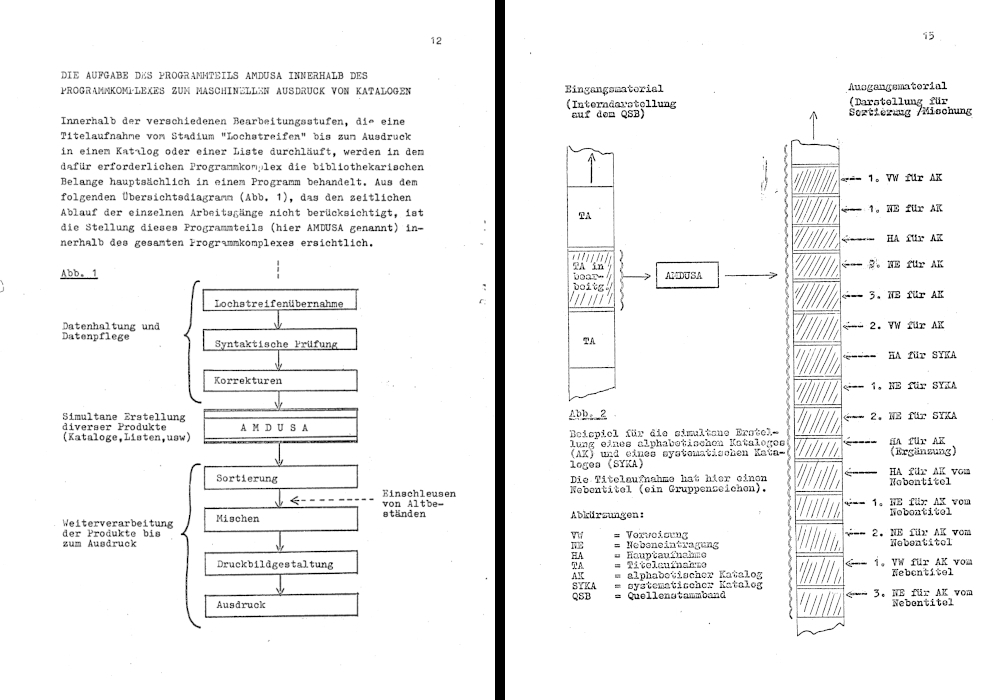
\includegraphics[width=.9\textwidth]{img/dg.jpg}
\caption{Beispiel einer schematischen Darstellung für ein datenbasiertes
System zum Ausdruck von Katalogen aus der internen Zeitschrift der
Bibliothek der Universität Konstanz. (Dg 1969: 12; Dg 1969:15) Solche
Darstellungen mussten 1969 in der bibliothekarischen Literatur -- nicht
nur solcher Vorreiter wie der Universität Konstanz -- nicht mehr erklärt
werden.}
\end{figure}

Erstaunlich schnell geht auch die Gründung von Institutionen, die sich
der Förderung von Computern in Bibliotheken widmen: 1963 wird im
Bibliotheksausschuss der DFG ein \enquote{Unterausschuss für Rationalisierung}
gegründet, welcher 1969 schon umbenannt ist in \enquote{Unterausschuss für
Datenverarbeitung} und zu diesem Zeitpunkt mehrere Projekte angestossen
und für deren Finanzierung gesorgt hat. (Lingenberg 1969) 1966 wird, wie
schon erwähnt, bei der Österreichischen Nationalbibliothek das \enquote{Institut
für Bibliotheksforschung} begründet, welches unter anderem die Aufgabe
der Förderung des Einsatzes von Computern hat. (Mayerhöfer 1966) In der
DDR wird 1967/68 vom betreffenden Ministerium ein
\enquote{Rationalisierungsprogramm für das wissenschaftliche Bibliothekswesen}
publiziert und für 1968 ein fertiger Plan für die Umsetzung desselben
angekündigt (Stein 1967), 1969 ist dann schon die weiter oben genannte
Arbeitsgruppe \enquote{EDAV in Bibliotheken} etabliert. (Ludwig 1969) Walter
Lingenberg erwähnt 1969, dass an der Staatsbibliothek Preussischer
Kulturbesitz, Berlin eine \enquote{Arbeitsstelle für Bibliothekstechnik}
eingerichtet würde (Lingenberg 1969: 2), was dann mit einiger Verspätung
1970 auch passierte (Arbeitsstelle für Bibliothekstechnik 1970). Während
also bis zur Mitte der 1960er über Rationalisierung im Bibliothekswesen
vor allem diskutiert und verschiedene mögliche Wege thematisiert wurden,
wird in der zweiten Hälfte des Jahrzehnt der Computer als Lösung
etabliert und auch institutionell verankert.\footnote{In ihrer
  Darstellung der Geschichte des Deutschen Bibliotheksinstituts, das
  nach Vorbereitungen 1978 gegründet wurde, erwähnt Helga Schwarz
  mehrfach Probleme des Instituts, Zugang zu einem Computer zu erlangen,
  um auf diesem Forschungsarbeiten durchzuführen. (Schwarz 2018) Sie
  führt nicht aus, welche Arbeiten dies genau waren, aber das
  Bibliotheksinstitut schloss damit explizit an Institutionen an, die
  schon in den 1960ern gegründet wurden, namentlich der \enquote{Arbeitsstelle
  für Bibliothekstechnik} an der Staatsbibliothek Preussischer
  Kulturbesitz, Berlin. Insoweit setzte sich hier eine Tradition an
  Fragestellungen fort.}

Damit ändern sich auch die Themen, die diskutiert werden. Es geht in den
letzten Jahren des Jahrzehnts vor allem darum, wie Computer effektiv
genutzt werden können und wie diese Computernutzung finanziert werden
kann. Dieses Problem wird sich in den folgenden Jahrzehnten durch die
rasante Entwicklung der Technik weg vom Mainframe-Computer lösen. In den
späten 1960er Jahren hingegen wird mehrfach die Forderung erhoben,
Rechenzentren zur gemeinsamen Nutzung von Computern zu bilden. (Möbus
1965; Schulte-Tigges 1965; Goltdammer 1967; Rationalisierungskomitees
für das dänische Volksbüchereiwesen 1967; Stein 1967; Kluth 1969)
Auffällig ist auch, dass zu Beginn des Jahrzehnts mehrfach betont wurde,
dass die Bibliotheken Aufgaben für ihre Nutzer*innen erfüllen sollen.
Walter Lingenberg -- der das gesamte Jahrzehnt über in diesem Kontext
aktiv war -- betonte 1963 noch folgendes:

\begin{quote}
\enquote{\ldots{} Rationalisierungsmaßnahmen {[}sollen{]} nicht dazu führen, daß
der Dienst am Benutzer verschlechtert wird.} (Lingenberg 1963: 348)
\end{quote}

Am Ende des Jahrzehnts wird über die Nutzer*innen nicht mehr diskutiert
-- was sichtbar wird, wenn die Texte von Lingenberg aus dieser Zeit
(Lingenberg 1967; 1968; 1969) dem von 1963 gegenübergestellt werden --,
sondern darüber, wozu Computer in der Bibliothek benutzt werden
können.\footnote{Einzige Ausnahme ist der Beitrag von Steinbuch (1968),
  der beklagt, dass die Technik schneller vorangeschritten sei, als das
  Verständnis der Menschen (oder Bibliotheken) von ihr und gleichzeitig
  in den Blick nimmt, dass in Zukunft Nutzer*innen direkt mit
  Informationstechnik umgehen werden, nicht nur die Bibliotheken.} Ohne
dass dies angestrebt war, scheint der Computer in gewisser Weise zum
Selbstzweck geworden zu sein.

\hypertarget{zu-kritik-utopie-und-die-bibliothek-der-zukunft}{%
\section{Zu Kritik, Utopie und die Bibliothek der
Zukunft}\label{zu-kritik-utopie-und-die-bibliothek-der-zukunft}}

Im Rückblick überraschend ist, dass in den 1960ern in der hier
herangezogenen Fachliteratur drei Themen kaum vorkommen: Kritik an
Rationalisierung oder Computereinsatz, utopische Vorstellungen und
Diskussionen darum, wie Bibliotheken in Zukunft aussehen sollen oder
werden. In einigen wenigen Texten finden sich Hinweise darauf, dass der
Einsatz von Maschinen den persönlichen Kontakt zwischen
Bibliothekar*innen und Nutzer*innen reduzieren könnte (Dux 1964; Pflug
1965) und ihr Einsatz realistisch und ohne überzogenen Hoffnungen
angegangen werden müsse (Baer 1964). Es scheint aber so, als wäre die
Grundhaltung zur Rationalisierung unter all denen, die sich an der
Literatur beteiligten, weitgehend ähnlich gewesen, obwohl gerade die
Einführung der Computer tatsächlich die Arbeit in Bibliotheken
veränderte: Sie wurde einfach als notwendig angesehen. Die dafür
eingesetzten finanziellen und personellen Ressourcen waren insbesondere
in der zweiten Hälfte der 1960er Jahre hoch, die Arbeit in Bibliotheken
wurde tatsächlich verändert, wenn beispielsweise Daten in
computerlesbarer Form aufgenommen wurden, nicht mehr auf Katalogkarten
-- und dennoch setzte dies wenig Nachdenken über die Zukunft oder gar
Kritik frei.

In wenigen Texten wird postuliert, dass sich die Bibliotheken zwar
verändern, aber auch in Zukunft weiter bestehen würden. (Loh 1965) Eine
der wenigen konkreten Utopien, die sich in diesen Texten findet, ist
dann bezeichnenderweise wenig phantasiereich und eher eine
Fortschreibung von Entwicklungen, nicht der Entwurf einer ganz anderen
Bibliothek (oder Welt):

\begin{quote}
\enquote{Der erst junge Traum, mit elektronischen datenverarbeitenden Maschinen
die Katalogherstellung, alle Katalogbefragungen und sämtliche
Buchungsarbeiten auf ein Minimum an körperlicher und geistiger Arbeit zu
reduzieren, wird früher oder später erfüllbar sein.} (Loh 1965: 385)
\end{quote}

Das ist überraschend, beschäftigen sich doch Bibliotheken hier mit der
gerade aktuellsten Technik, die mit grossen Versprechen über ihre
zukünftige Leistungsfähigkeit verbunden war und die gleichzeitig von
Teilen der Gesellschaften im DACH-Raum heftig kritisiert wurde. (Müller
\& Nievergelt 1996) Nicht zu vergessen ist, dass sich die Gesellschaften
im DACH-Raum in diesem Jahrzehnt an sich massiv veränderten, vor allem
liberaler wurden und radikal alternative Gesellschaftsentwürfe,
inklusive rabiater politischer Kritik des gesellschaftlichen Status Quo,
zumindest in der BRD, Österreich und Schweiz, nicht selten waren. All
dies findet sich in der Literatur zur Rationalisierung und
Automatisierung von Bibliotheken nicht wieder. Offenbar existierte in
dieser ein breiter Konsens dazu, dass sich die Arbeit in Bibliotheken
verändern und man dafür Computer nutzen müsse. Diskutiert wurde nur, wie
genau. Ein wenig erscheint im Rückblick diese Entwicklung in
Bibliotheken inhaltlich losgelöst von der Gesellschaft gewesen zu sein.

\hypertarget{unterschiede-zwischen-den-luxe4ndern}{%
\section{Unterschiede zwischen den
Ländern}\label{unterschiede-zwischen-den-luxe4ndern}}

Während sich zum hier behandelten Thema aus den 1960er Jahren nur wenige
Beiträge aus der Schweiz (wo die Diskussion etwas später einzusetzen
scheint) und Österreich (wo die Nationalbibliothek in Wien tonangebend
zu sein scheint) finden lassen und es deshalb schwierig ist, diese
direkt zu vergleichen, lässt sich an den unterschiedlichen Beiträgen aus
BRD und DDR zeigen, dass sich Bibliothekswesen -- auch wenn sie in
diesem Fall erst rund zwanzig Jahre getrennte Wege gingen --
unterschiedlich entwickeln, selbst wenn sie ähnliche Herausforderungen
(Wachstum der Literatur, der Anforderungen und der Nutzer*innenzahl)
angehen und dabei ähnliche Lösungen (Rationalisierung, Einsatz von
Computern) wählen. Die Gesellschaft und Strukturen eines Landes haben
offensichtlich einen grossen Einfluss auf das Bibliothekswesen.

In der DDR wird schnell versucht, Rationalisierung und dann den Einsatz
von datenverarbeitenden Maschinen theoretisch zu fassen. Immer wieder
werden neue Definitionen gegeben, an schon vorhandene Theorien oder
politische Vorgaben, die als Theorie behandelt werden (Schulze 1964),
angeschlossen, auf Normungen gedrängt (Goltdammer 1967) und darauf
geachtet, welche Terminologie sich entwickelt oder entwickeln sollte.
(Dux \& Siewert 1965; Lohse 1966) Zudem wird immer wieder für das
gesamte Bibliothekswesen des Landes, zumindest das Wissenschaftliche,
geplant, nicht für einzelne Bibliotheken. (Stein 1967; Ludwig 1969)

Auf der einen Seite ist diese theoretische Beschäftigung wohl zu
erklären mit den geringeren Mitteln für die Anschaffung von Computern
und damit auch dem schwierigeren Zugang zu ihnen. So gesehen ist die
Theoretisierung immer auch Vorarbeit für den Zeitpunkt, an dem Computer
zur Verfügung stehen werden. Auf der anderen Seite sind sie aber dem
Vorgehen bei allen Veränderungen in der DDR (und anderen sozialistischen
Staaten) inhärent: Da die Gesellschaft auf konkreter, fortlaufender
Planung aufgebaut sein sollte, die auf einer theoretischen Basis
aufbaute, war es auch nur folgerichtig, dass Bibliotheken die
Rationalisierung ihrer Arbeit auf diese Weise angingen. Deshalb ist zum
Beispiel die Terminologie auch wichtig, da nur mit ihr sinnvoll
Theorieentwicklung betrieben werden kann. Weil zudem -- zumindest
idealtypisch -- alle Wissenschaftlichen Bibliotheken als Teil von
zusammenhängenden Netzen verstanden wurden, war es folgerichtig, für
alle Bibliotheken eines Typus zugleich zu planen.

Hingegen zeichnet sich die Entwicklung in der BRD durch vielfältige
Ansätze und Projekte, aber vor allem durch eine hohe
Praxisorientiertheit aus. Theoretische Auseinandersetzungen gab es nur
am Rande und am Beginn der hier beschriebenen Prozesse (Lingenberg
1963), eine eigene Theorieentwicklung gab es nicht. Ebenso wenig
existierte eine übergreifende Planung. Vielmehr gingen Bibliotheken an
mehreren Orten schnell daran, eigene Projekte umzusetzen, die allesamt
als Vorbild für andere Bibliotheken dienen konnten (so wurde dann auch
über sie berichtet), die aber zuvörderst in der jeweiligen Bibliothek
funktionierten.

Zum Teil lässt sich dies -- im Gegensatz zur Situation in der DDR --
wohl mit den tatsächlich vorhandenen finanziellen Mitteln erklären, die
recht früh für die Anschaffung von Computern zur Verfügung standen.
Insoweit konnten Bibliotheken in der BRD schneller dazu übergehen,
tatsächlich mit ihnen zu arbeiten und an ihnen zu lernen. Zum anderen
Teil aber spiegelt sich hier auch die Struktur der Gesellschaft wieder,
die eher in Einzelinstitutionen, welche in Konkurrenz zueinander stehen,
organisiert ist. Kooperation muss dann anders bewerkstelligt werden
(unter anderem über den Bibliotheksausschuss in der DFG) und ist nicht
schon in einem Netz aller Bibliotheken angelegt.

\hypertarget{fazit}{%
\section{Fazit}\label{fazit}}

Der in diesem Text dargebotene Überblick über die Integration der ersten
Computer in die Bibliothekswesen im DACH-Raum bietet eine Blaupause, um
Veränderungen in Bibliotheken zu analysieren, auch heute, wo andere
Themen -- Forschungsdatenmanagement, Open Science in Wissenschaftlichen
Bibliotheken oder Partizipation und der Einsatz von Technik wie Robotern
in Öffentlichen Bibliotheken -- im Fokus stehen. Die Geschichte
wiederholt sich nicht einfach, aber Strukturen, denen Institutionen bei
ihren Entwicklungen pfadabhängig folgen, existieren weiterhin.

Auffällig ist zuerst, dass die Entwicklung im Rückblick rasend schnell
vonstatten ging. (Pflug 1969) Innerhalb eines Jahrzehnts wurde von einer
wahrgenommenen Krise -- steigende Literaturproduktion, nicht
mitwachsendes Personal -- zum konkreten Einsatz von Maschinen in
Bibliotheken übergegangen. Ebenso wurde innerhalb dieses Jahrzehnts von
ersten terminologischen Einführungen zur konkreten Darstellung von
Datenstrukturen übergegangen, die zu diesem Zeitpunkt offenbar allgemein
verstanden wurden. Auch wenn in einigen Texten vom Scheitern von
Projekten, überzogenen Erwartungen oder einem gewissen
Strukturkonservatismus von Bibliotheken berichtet wird (Pflug 1965; Ra
1969) -- und wohl von den Handelnden auch als Ausbremsen von Veränderung
verstanden wurden --, gab es eine kontinuierliche Entwicklung, die das
Gegenteil zeigte. Innerhalb von nicht einmal zehn Jahren waren neue
Maschinen und Arbeitsstrukturen etabliert. Am Anfang der 1960er Jahre
machten sich Bibliotheken Gedanken darüber, wie ihre Arbeitsprozesse
rationalisiert werden könnten, am Ende des Jahrzehnts war es dann zum
Beispiel in vielen Bibliotheken schon etablierte Praxis, die
Katalogisierung computergestützt zu bewerkstelligen und regelmässig
Kataloge auszudrucken. (Vogt 1967; Margot \& Monnier 1968; Niewalda \&
Preuß 1969) Diese reale Veränderung ging in der alltäglichen Praxis
vielleicht unter, im Rückblick ist sie aber erstaunlich und deutet
darauf hin, dass Bibliotheken sehr wohl in der Lage sind, sich zu
entwickeln und zeitgemässe Lösungen für Herausforderungen zu finden.

Gleichzeitig ist bei dieser Geschichte auffällig, wie sehr die
Bibliothek und ihre Organisation im Mittelpunkt der Diskussionen und
Projekte stand. Es gab anfänglich immer wieder Verweise darauf, dass
Bibliotheken auf Entwicklungen, die ausserhalb ihrer selbst stattfinden
-- wissenschaftlich-technische Revolution, steigende Literaturproduktion
-- reagieren müssten und dass sie ihre Aufgaben vor allem für ihre
Nutzer*innen erfüllen. Aber am Ende ging es immer darum, die Arbeit in
der Bibliothek zu organisieren und zu verändern. So wurde in all den
hier ausgewerteten Texten kein einziges Mal die Perspektive der
Nutzer*innen oder anderer beteiligter Institutionen -- der
Hochschulleitungen, der Finanziers wie der DFG oder dem Ministerium für
Hoch- und Fachschulwesen -- einbezogen oder diese gar abgefragt. Erwähnt
wurde weiter oben auch, dass die gesellschaftlichen Entwicklungen dieser
Jahre keinen Widerhall bei diesen Entwicklungen in Bibliotheken gefunden
zu haben scheinen. Bibliotheken entwickelten sich vor allem mit Bezug
auf sich selber und auf andere Bibliotheken weiter. Für die Bewertung
heutiger Entwicklungen in Bibliotheken ergibt sich daraus die Frage, wie
dies real gestaltet ist: Auch heute erheben Bibliotheken den Anspruch,
auf Entwicklungen ausserhalb ihrer selbst zu reagieren und gleichzeitig
die eigene Arbeit zu leisten, um Anforderungen der Nutzer*innen und
anderer Institutionen zu erfüllen. Aber ist die Entwicklung wirklich
darauf bezogen oder folgt sie doch eher internen Logiken des
Bibliothekswesens selber?

Erstaunlich war bei der geschilderten Entwicklung, wie rasant sich die
anfänglich breite Diskussion darauf zuspitzte, Computer als Lösung in
den Mittelpunkt zu stellen. Am Ende des Jahrzehnts wurde nicht mehr
begründet, warum Computer eingesetzt werden sollten und auch kaum mehr
auf mögliche Rationalisierungsmöglichkeiten eingegangen, sondern fast
nur noch diskutiert, wie genau die bibliothekarische Arbeit um Computer
herum organisiert werden müsste. Die Maschine war damit in gewisser
Weise zum Selbstzweck geworden. Einher ging dies, wie auch schon
erwähnt, mit einer erstaunlichen Utopielosigkeit. Die Fokussierung auf
den Einsatz von Computern ging damit einher, dass zumindest in
publizierter Form nicht mehr über Alternativen nachgedacht wurde.
Eventuell ist dies ein Effekt der als zu viel wahrgenommen Arbeit in
Bibliotheken zu verstehen: Wenn die Ressourcen und die Arbeitszeit schon
vollständig für den Alltag und die Lösung einzelner Projekte verwendet
wird und sich am Horizont immer mehr und nicht enden wollende Arbeit
abzeichnet, lässt sich vielleicht schwer ein Ort und die Zeit finden,
über andere mögliche Entwicklungen nachzudenken. Aber das führt dann
dazu, dass ohne weitere Prüfung auf einem einmal eingeschlagenen Weg
weitergegangen wird.

Grundsätzlich zeigt diese Geschichte auch, dass Bibliotheken zwar nicht
die Avantgarde beim Einsatz von Technik oder anderen Veränderungen
darstellen -- dass sie also zum Beispiel nicht die Forschung zur
Entwicklung von datenverarbeitenden Maschinen durchführten --, aber dass
sie doch kurz hinter dieser Avantgarde folgend sehr schnell
Entwicklungen aufnehmen und integrieren können. Das Problem ist nicht
ein angeblicher Strukturkonservatismus der Bibliotheken. Problematischer
scheint eher, dass die Lösungen schnell alternativlos zu werden
scheinen. Unter der erstaunlichen Betriebsamkeit von Bibliotheken, die
sich in den 1960ern zeigte, scheint die Kreativität und die Reflexion
über einmal eingeschlagene Entwicklungsrichtungen zu verschwinden. Zu
fragen wäre, ob dies nur für dieses Thema gilt oder ob dies eine
allgemeine Struktur von Entwicklungen im Bibliothekswesen darstellt.

\hypertarget{literatur}{%
\section{Literatur}\label{literatur}}

Arbeitsstelle für Bibliothekstechnik. (1970). \emph{Bericht über den
Aufbau und die Arbeiten der ABT: In den Jahren 1970-1972}. ABT.

Baer, H. (1964). Bibliothek, Fachbibliothek, Dokumentation: Vom Katalog
zum Automatic Information System. \emph{Nachrichten / Vereinigung
Schweizerischer Bibliothekare, Schweizerische Vereinigung für
Dokumentation}, \emph{40}(3), 65--81.

Bührer, G. (1966). Die Mechanisierung von Akzession und Ausleihe: In der
McKeldin Library, University of Maryland, College Park, Maryland 20742,
USA. \emph{Nachrichten / Vereinigung Schweizerischer Bibliothekare,
Schweizerische Vereinigung für Dokumentation}, \emph{42}(4), 121--128.

Dg. (1969). Die Aufgabe des Programmteils AMDUSA innerhalb des
Programmkomplexes zum maschinellen Ausdruck von Katalogen.
\emph{Bibliothek aktuell: Informationsblatt für die Mitarbeiter des
Bibliothek der Universität Konstanz}, \emph{1}(3), 12--15.

Dux, W. (1964). Fragen der Technisierung von Bibliotheken.
\emph{Zentralblatt für Bibliothekswesen}, \emph{78}(6), 321--339.

Dux, W. (1966). Zur gegenwärtigen und zukünftigen Bedeutung der
Reprographie für die wissenschaftlichen Bibliotheken. \emph{Zentralblatt
für Bibliothekswesen}, \emph{80}(8), 455--467.

Dux, W., \& Siewert, T. (1965). Symposium über Informationstechnik Juni
1965 Moskau. \emph{Zentralblatt für Bibliothekswesen}, \emph{79}(10),
608--614.

Fock, J. (1967). Das Lochkartenverfahren in der Leihstelle der Staats-
und Universitätsbibliothek Hamburg. \emph{Zeitschrift für
Bibliothekswesen und Bibliographie}, \emph{14}(3), 143--153.

Glagla, H. (1966). Maschinelle Datenverarbeitung in der Buchausleihe der
Staats- und Universitäts-Bibliothek (SUB) Hamburg. \emph{Zeitschrift für
Bibliothekswesen und Bibliographie}, \emph{13}(3), 169--177.

Goltdammer, I. (1967). Die Rationalisierung der Arbeit in
wissenschaftlichen Bibliotheken: Internationale wissenschaftliche Tagung
des Methodischen Zentrums für wissenschaftliche Bibliotheken beim
Staatssekretariat für das Hoch- und Fachschulwesen am 8. und 9. Juni
1967 in Berlin. \emph{Zentralblatt für Bibliothekswesen}, \emph{81}(1),
667--675.

Höhne, H. (1963). Zur Rationalisierung der Arbeit in den
wissenschaftlichen Bibliotheken. \emph{Zentralblatt für
Bibliothekswesen}, \emph{77}(3), 112--120.

Jordi, L. (1970). L'information scientifique et technique en URSS:
Rapport sur un voyage d'études, septembre 1969 . \emph{Nachrichten /
Vereinigung Schweizerischer Bibliothekare, Schweizerische Vereinigung
für Dokumentation}, \emph{46}(6), 251--256.
\url{https://doi.org/10.5169/SEALS-771121}

Kluth, R. (1969). Elektronische Datenverarbeitung in Bibliotheken.
\emph{Bibliotheksdienst}, \emph{3}(7), 21--26.

Kuttner, S. (2018). \enquote{Funktionär im Räderwerk des Betriebs}:
Bibliothekarisches Berufsbild und Modernekritik in der späten
Nachkriegszeit. In S. Kuttner \& K. Kempf (Hrsg.), \emph{Buch und
Bibliothek im Wirtschaftswunder: Entwicklungslinien, Kontinuitäten und
Brüche in Deutschland und Italien während der Nachkriegszeit
(1949-1965)} (S. 65--71). Harrassowitz Verlag.

Lingenberg, W. (1963). Bemerkungen zu Problemen der Datenverarbeitung in
der Katalog- und Verwaltungspraxis der Bibliotheken. \emph{Zeitschrift
für Bibliothekswesen und Bibliographie}, \emph{10}(6), 346--354.

Lingenberg, W. (1967). Über das Arbeiten mit Lochstreifen bei speziellen
Bibliotheksproblemen. \emph{Zeitschrift für Bibliothekswesen und
Bibliographie}, \emph{14}(1), 8--14.

Lingenberg, W. (1968). Mechanisierung und Automatisierung in
Amerikanischen Bibliotheken 1967. \emph{Zeitschrift für Bibliothekswesen
und Bibliographie}, \emph{15}(3), 143--185.

Lingenberg, W. (1969). Computereinsatz in Bibliotheken der
Bundesrepublik Deutschland. \emph{Zeitschrift für Bibliothekswesen und
Bibliographie}, \emph{16}(1), 1--23.

Loh, G. (1965). Stand und Möglichkeiten der Anwendung von manuellen
Lochkartenverfahren im wissenschaftlichen Bibliothekswesen.
\emph{Zentralblatt für Bibliothekswesen}, \emph{79}(7), 385--403.

Lohse, H. (1966). Die Verwendung der Begriffe Arbeitsproduktivität,
produktive Arbeit und technisch begründete Arbeitsnormen in
wissenschaftlichen Bibliotheken. \emph{Zentralblatt für
Bibliothekswesen}, \emph{80}(1), 22--33.

Ludwig, R. (1969). Die einheitliche Einsatzvorbereitung von
elektronischen Datenverarbeitungsanlagen im Bibliothekswesen und die
Arbeitsgruppe \enquote{EDVA in Bibliotheken}. \emph{Zentralblatt für
Bibliothekswesen}, \emph{83}(8), 438--447.

Margot, J.-M., \& Monnier, J.-F. (1968). BITRA: Système pour l'Édition
automatique d'un catalogue de bibliothèque. \emph{Nachrichten /
Vereinigung Schweizerischer Bibliothekare, Schweizerische Vereinigung
für Dokumentation}, \emph{44}(2), 33--37.

Mayerhöfer, J. (1966). Österreichisches Institut für
Bibliotheksforschung. \emph{Biblios}, \emph{15}(2), 125--129.

Mayerhöfer, J. (1982). 15 Jahre Österreichisches Institut für
Bibliotheksforschung, Dokumentations- und Informationswesen.
\emph{Biblios}, \emph{31}(2), 117--136.

Möbus, R. (1965). Bibliothekstechnik auf der Leipziger Jubiläumsmesse.
\emph{Zentralblatt für Bibliothekswesen}, \emph{79}(7), 429--432.

Mojek. (1967). Elektronische Datenverarbeitung bei der Stadtbücherei
Duisburg. \emph{Bibliotheksdienst} \emph{1}(3), 16--18.

Mullaney, T. S. (2017). \emph{The Chinese typewriter a history}. The MIT
Press.

Müller, C., \& Nievergelt, B. (1996). \emph{Technikkritik in der Moderne
Empirische Technikereignisse als Herausforderung an die
Sozialwissenschaft} (1st ed.~1996.). VS Verlag für Sozialwissenschaften.
\url{https://doi.org/10.1007/978-3-322-97332-0}

Niewalda, P., \& Preuß, G. (1969). Die Elektronik im Dienste der
Katalogisierung der Universitätsbibliothek Regensburg: Ein
Erfahrungsbericht. \emph{Zeitschrift für Bibliothekswesen und
Bibliographie}, \emph{16}(2), 86--118.

Pflug, G. (1965). Probleme der elektronischen Datenverarbeitung in
Bibliotheken. \emph{Libri}, \emph{15}(1--4), 35--49.
\url{https://doi.org/10.1515/libr.1965.15.1-4.35}

Pflug, G. (Hrsg.). (1967). \emph{Mechanisierung und Automatisierung in
Amerikanischen Bibliotheken: Eindrücke einer Studienreise Deutscher
Bibliothekare im Frühjahr 1965}. Vittorio Klostermann.

Pflug, G. (1969). New Steps in Library Automation in the Federal
Republic of Germany. \emph{Libri}, \emph{19}(1--4), 304--312.
\url{https://doi.org/10.1515/libr.1969.19.1-4.304}

Pietsch, E. H. E. (1962). Die künftige Entwicklung der Dokumentation.
\emph{Libri}, \emph{12}(4), 287--319.
\url{https://doi.org/10.1515/LIBR.1962.12.4.287}

Ra. (1969). Ein gewisses Unbehagen an der Datenverarbeitung.
\emph{Bibliothek aktuell: Informationsblatt für die Mitarbeiter des
Bibliothek der Universität Konstanz}, \emph{1}(3), 7.

Rationalisierungskomitees für das dänische Volksbüchereiwesen. (1967).
\emph{Rationalisierung der öffentlichen Büchereien Dänemarks: Gutachten
des Rationalisierungskomitees des Dänischen Bibliotheksverbandes.
Deutsche Übersetzung und Bearbeitung von Friedrich Ochsner} (H.
Süberkrüb, Hrsg.; F. Ochsner, Übers.). Otto Harrassowitz.

Rittberger, W. (1964). Bibliotheksrationalisierung mit
Lochstreifengeräten. \emph{Zeitschrift für Bibliothekswesen und
Bibliographie}, \emph{11}(2), 77--85.

Scherrer-Bylund, P. (1968). Tradition und Technik in den Bibliotheken.
\emph{Zeitschrift für Bibliothekswesen und Bibliographie},
\emph{15}(5/6), 307--323.

Schulte-Tigges, F. (1965). Integrierte Datenverarbeitung in der
Bibliothek. \emph{Libri}, \emph{15}(1--4), 23--34.
\url{https://doi.org/10.1515/libr.1965.15.1-4.23}

Schulte-Tigges, Friedhelm. (1963). Die Anwendung elektronischer
Datenverarbeitender Maschinen in einzelnen Bereichen des
Bibliothekswesens. \emph{Zeitschrift für Bibliothekswesen und
Bibliographie}, \emph{10}(6), 331--345.

Schulze, H. (1964). Bemerkungen zur Arbeitsproduktivität in
wissenschaftlichen Fachbibliotheken. \emph{Zentralblatt für
Bibliothekswesen}, \emph{78}(2), 82--88.

Schwarz, G. (1967). Zur Rationalisierung im Wissenschaftlichen
Bibliothekswesen. \emph{Zentralblatt für Bibliothekswesen},
\emph{81}(11), 641--651.

Schwarz, H. (2018). \emph{Das Deutsche Bibliotheksinstitut: Im
Spannungsfeld zwischen Auftrag und politischen Interessen}. Simon Verlag
für Bibliothekswissen.

Stamm, E. (1963). Programmierkurs für Dokumentare und Bibliothekare im
Deutschen Rechenzentrum Darmstadt vom 25.3. bis 5.4. und 6.5. bis
17.5.1963. \emph{Zeitschrift für Bibliothekswesen und Bibliographie},
\emph{10}(6), 371--372.

Stein, G. (1967). Elektronische Datenverarbeitung in wissenschaftlichen
Bibliotheken. \emph{Zentralblatt für Bibliothekswesen}, \emph{81}(11),
651--666.

Steinbuch, K. (1968). Zukunftsaufgaben der Informationstechnik im
Hinblick auf das Bibliothekswesen. \emph{Zeitschrift für
Bibliothekswesen und Bibliographie}, \emph{15}(5/6), 291--306.

Steininger, F. (1970). \emph{Amerikanische Bibliotheken: Große Aufgaben,
neue Mittel, aufwendige Experimente\,; Eindrücke einer Studienreise
September bis Dezember 1969}. Österreichisches Institut für
Bibliotheksforschung.

Stummvoll, J. (1969). \emph{Elektronik in Bibliotheken: Kritische
Auseinandersetzung mit Kritiken an der Studie \enquote{Die Bibliothek der
Zukunft}}. Österreichische Nationalbibliothek.

Stummvoll, J., \& Mayerhöfer, J. (1972). \emph{Das Österreichische
Institut für Bibliotheksforschung, Dokumentations- u. Informationswesen
(ÖIBF)}.

Süberkrüb, H., \& Hoffmann, K.-D. (1967). Vorwort der Herausgeber. In H.
Süberkrüb \& K.-D. Hoffmann (Hrsg.), \emph{Rationalisierung der
öffentlichen Büchereien Dänemarks: Gutachten des
Rationalisierungskomitees des Dänischen Bibliotheksverbandes. Deutsche
Übersetzung und Bearbeitung von Friedrich Ochsner} (S. 9). Otto
Harrassowitz.

Sydler, J.-P. (1970). Aspects de l'automation dans les bibliothèques
américaines: Rapport sur un voyage d'études aux Etats-Unis, avril-mai
1970 {[}Text/html,application/pdf{]}. \emph{Nachrichten / Vereinigung
Schweizerischer Bibliothekare, Schweizerische Vereinigung für
Dokumentation}, \emph{46}(5), 181--189.
\url{https://doi.org/10.5169/SEALS-771116}

Taube, Dr.~(1963). Rationalisierungsprobleme im großstädtischen
Büchereiwesen. \emph{Büchereidienst}, \emph{3}(8), ohne Seiten.

Universitätsbibliothek Bochum (Hrsg.). (1967). \emph{Die automatische
Buchausleihe: Erfahrungen in der Universitätsbibliothek Bochum}.
Universitätsbibliothek Bochum.

Vogt, H. (1967). Die automatisierte Katalogisierung von Zeitschriften
und Serien an der Niedersächsischen Staats- und Universitätsbibliothek
in Göttingen. \emph{Zeitschrift für Bibliothekswesen und Bibliographie},
\emph{14}(3), 125--142.

von Kortzfleisch, H. (1968). Rationalisierungsreserven in
wissenschaftlichen Bibliotheken: Die wissenschaftliche Bibliothek aus
betriebswirtschaftlicher Sicht. \emph{Zeitschrift für Bibliothekswesen
und Bibliographie}, \emph{15}(5/6), 324--339.

Wegmüller, F., \& Hoffmann-La Roche, F. (1970). Elektronische
Datenverarbeitung in Bibliotheken: Bericht über das UNESCO-Seminar in
Regensburg, 13.-18. April 1970. \emph{Nachrichten / Vereinigung
Schweizerischer Bibliothekare, Schweizerische Vereinigung für
Dokumentation}, \emph{46}(5), 189--202.
\url{https://doi.org/10.5169/SEALS-771117}

Zimmermann, G. (1965). Der Weinberg-Report und die schweizerische
Dokumentation . \emph{Nachrichten / Vereinigung Schweizerischer
Bibliothekare, Schweizerische Vereinigung für Dokumentation},
\emph{41}(2), 33--37. \url{https://doi.org/10.5169/SEALS-771206}

%autor
\begin{center}\rule{0.5\linewidth}{0.5pt}\end{center}

\textbf{Karsten Schuldt} ist Wissenschaftlicher Mitarbeiter am
Schweizerischen Institut für Informationswissenschaft, FH Graubünden und
Redakteur der LIBREAS. Library Ideas.

\end{document}
